\documentclass[12pt,ngerman,parskip=half]{scrartcl}

\usepackage{babel}
\usepackage{tikz}
\usepackage{blindtext}

\begin{document}

\blindtext

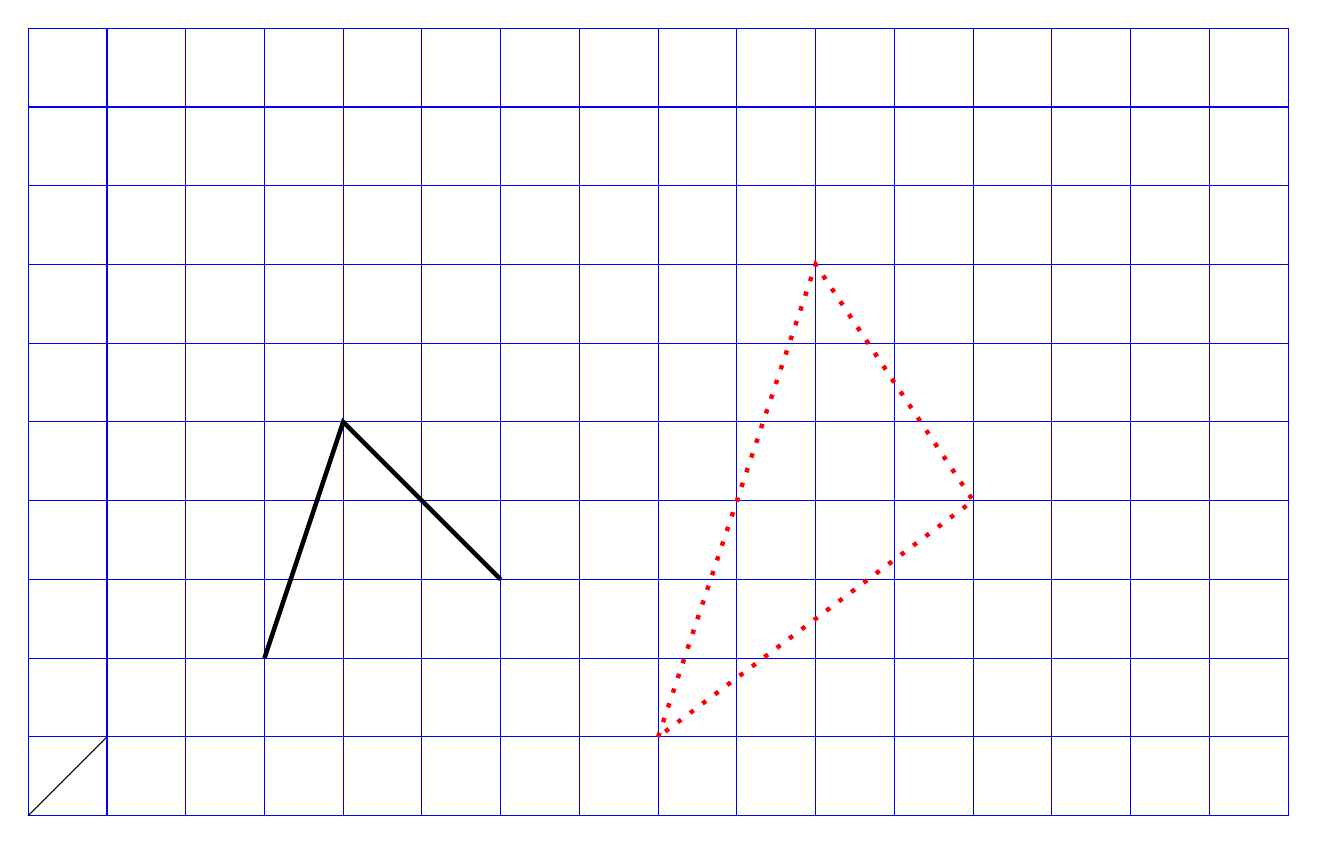
\begin{tikzpicture}
\draw [step=1cm,blue,thin] (0,0) grid (16,10);
\draw (0,0) -- (1,1);
\draw[ultra thick] (3,2) -- (4,5) -- (6,3);
\draw[red,ultra thick,loosely dotted] (8,1) -- (10,7) -- (12,4) -- cycle;
\end{tikzpicture}

\blindtext


\blindtext

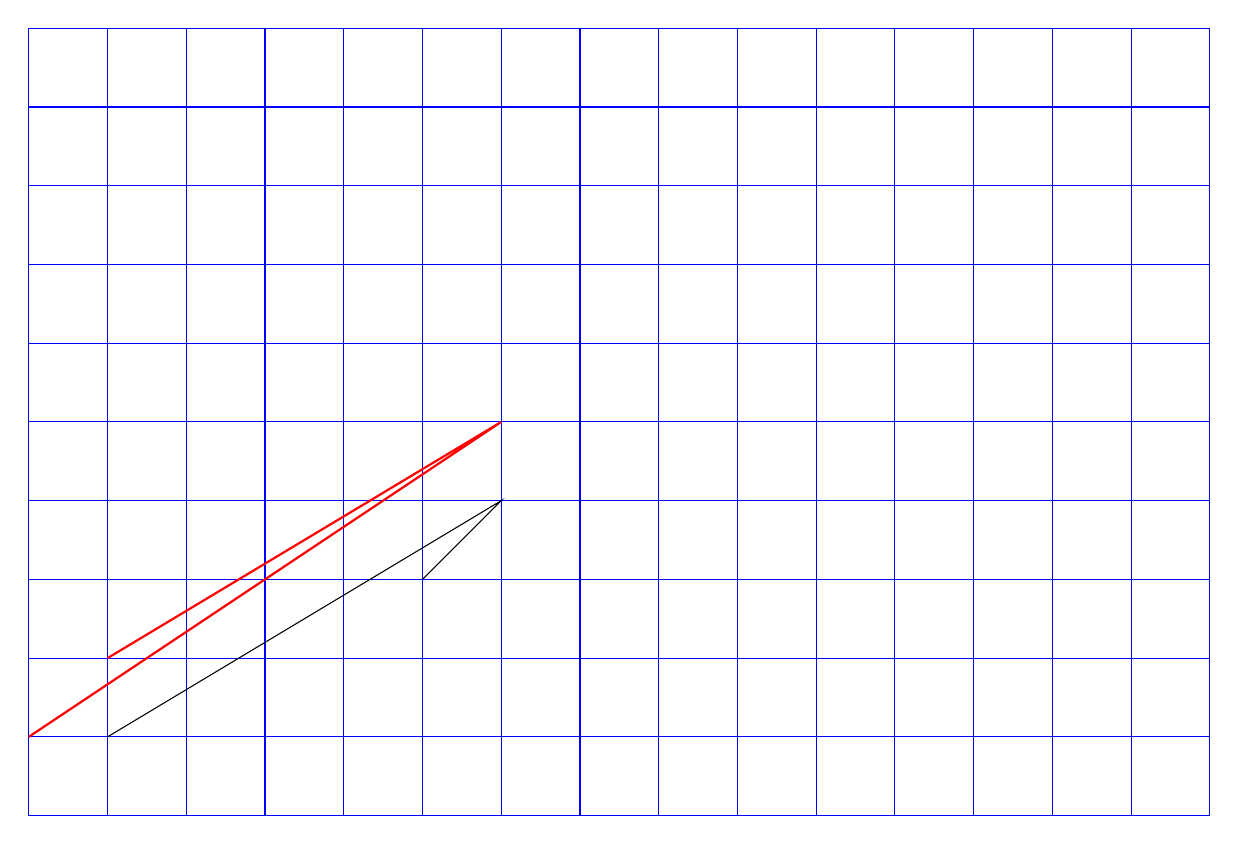
\begin{tikzpicture} % Achtung:_ kann leicht zum Haareraufen führen!
\draw [step=1cm,blue,thin] (0,0) grid (15,10);
\draw(1,1) -- ++(5,3) -- ++(-1,-1) ; % relative Koordinaten mit ++ mit Koordinatenupdate!
\draw[red,thick](1,2) -- +(5,3) -- +(-1,-1) ; % relative Koordinaten mit ++ ohne  Koordinatenupdate!
\end{tikzpicture}

\blindtext

\end{document}